\documentclass[11pt,twocolumn]{article}
\usepackage[utf8]{inputenc}
\usepackage{amsmath,amssymb,amsthm}
\usepackage{graphicx}
\usepackage{booktabs}
\usepackage{algorithm}
\usepackage{algorithmic}
\usepackage{hyperref}
\usepackage{xcolor}
\usepackage{listings}
\usepackage{tikz}
\usetikzlibrary{shapes,arrows,positioning,fit,backgrounds,calc}
\usepackage[margin=1in]{geometry}
\usepackage{enumitem}
\usepackage{tabularx}
\usepackage{multirow}
\usepackage{subcaption}

\definecolor{codegreen}{rgb}{0,0.6,0}
\definecolor{codegray}{rgb}{0.5,0.5,0.5}
\definecolor{codepurple}{rgb}{0.58,0,0.82}
\definecolor{backcolour}{rgb}{0.95,0.95,0.92}

\lstdefinestyle{mystyle}{
    backgroundcolor=\color{backcolour},
    commentstyle=\color{codegreen},
    keywordstyle=\color{codepurple},
    numberstyle=\tiny\color{codegray},
    stringstyle=\color{codegreen},
    basicstyle=\ttfamily\footnotesize,
    breakatwhitespace=false,
    breaklines=true,
    captionpos=b,
    keepspaces=true,
    numbers=left,
    numbersep=5pt,
    showspaces=false,
    showstringspaces=false,
    showtabs=false,
    tabsize=2
}
\lstset{style=mystyle}

\newtheorem{definition}{Definition}
\newtheorem{theorem}{Theorem}
\newtheorem{lemma}{Lemma}
\newtheorem{proposition}{Proposition}

\title{Hanzo LLM Gateway: Unified Proxy Architecture\\for 100+ AI Provider Integration}
\author{Hanzo AI Research\\
\texttt{research@hanzo.ai}\\
\textit{Hanzo AI \quad San Francisco, CA}}
\date{February 2026}

\begin{document}

\maketitle

\begin{abstract}
The proliferation of large language model (LLM) providers---each with incompatible APIs, pricing models, rate limits, and capability profiles---creates a fragmentation problem for production AI systems. We present the Hanzo LLM Gateway, a unified proxy that normalizes access to over 100 AI providers behind a single OpenAI-compatible API surface. The gateway implements intelligent request routing via a multi-objective optimization framework that balances latency, cost, and quality. Key contributions include: (1) a streaming-aware load balancer with provider health tracking and automatic failover, (2) a semantic cache achieving 34\% cache hit rates on production workloads with sub-2ms lookup latency, (3) a cost attribution engine with per-token accounting across heterogeneous pricing models, and (4) a fallback chain mechanism that transparently retries across providers while preserving streaming semantics. In production at Hanzo AI serving 2.8 billion tokens monthly, the gateway reduces median latency by 23\% through intelligent routing, cuts costs by 31\% via caching and model selection, and achieves 99.97\% availability through multi-provider redundancy. We release the gateway as open-source software under the Apache 2.0 license.
\end{abstract}

\section{Introduction}

The landscape of large language model providers has expanded dramatically since the release of GPT-3 in 2020~\cite{brown2020language}. As of early 2026, production AI systems may need to integrate with OpenAI, Anthropic, Google DeepMind, Meta, Mistral, Cohere, Together AI, Fireworks, Groq, AWS Bedrock, Azure OpenAI, and dozens of additional providers~\cite{bommasani2022opportunities}. Each provider exposes a distinct API surface with incompatible request formats, authentication schemes, rate limiting policies, error codes, and streaming protocols.

This fragmentation imposes substantial engineering overhead. A survey of 340 AI engineering teams revealed that 67\% maintain separate integration code for three or more providers, 43\% have experienced production outages due to single-provider dependencies, and the median time to integrate a new provider is 2.3 engineering-weeks~\cite{aiinfra2025survey}. Beyond integration complexity, teams face the multi-objective optimization problem of selecting the optimal provider for each request given constraints on latency, cost, quality, and compliance.

The Hanzo LLM Gateway addresses these challenges through a proxy architecture that:

\begin{enumerate}[leftmargin=*]
    \item \textbf{Normalizes} all provider APIs to a single OpenAI-compatible interface, including chat completions, embeddings, image generation, audio transcription, and function calling.
    \item \textbf{Routes} requests intelligently across providers using a configurable policy engine that optimizes for latency, cost, quality, or custom objectives.
    \item \textbf{Caches} responses at the semantic level, recognizing equivalent prompts despite surface-level variation.
    \item \textbf{Tracks} costs with per-token granularity across heterogeneous pricing models including per-token, per-request, per-minute, and reserved capacity pricing.
    \item \textbf{Fails over} transparently across providers while maintaining streaming connections and preserving partial responses.
\end{enumerate}

\paragraph{Contributions.} This paper makes the following contributions:
\begin{itemize}[leftmargin=*]
    \item A formal model for multi-provider LLM routing as a multi-objective optimization problem with latency, cost, and quality objectives (Section~\ref{sec:routing}).
    \item A streaming-aware load balancer with exponentially weighted health scores and circuit breaker patterns (Section~\ref{sec:loadbalancing}).
    \item A semantic caching layer using locality-sensitive hashing for prompt equivalence detection, achieving 34\% hit rates with 97.2\% precision (Section~\ref{sec:caching}).
    \item A cost attribution engine supporting 14 distinct pricing models with sub-cent accuracy (Section~\ref{sec:cost}).
    \item A comprehensive evaluation on production traffic from 2.8B monthly tokens across 127 provider endpoints (Section~\ref{sec:evaluation}).
\end{itemize}

\section{Background and Related Work}
\label{sec:background}

\subsection{LLM Provider Landscape}

The LLM provider ecosystem can be categorized along several dimensions. \textit{First-party providers} (OpenAI, Anthropic, Google) train and serve their own models. \textit{Cloud providers} (AWS Bedrock, Azure OpenAI, Google Vertex AI) offer managed access to both first-party and third-party models. \textit{Inference platforms} (Together AI, Fireworks, Groq, Replicate) specialize in serving open-weight models with optimized infrastructure. \textit{Self-hosted solutions} (vLLM~\cite{kwon2023vllm}, TGI~\cite{tgi2023}, Ollama) enable on-premises deployment.

Each category exhibits distinct operational characteristics. First-party providers offer the highest model quality but with opaque capacity management. Cloud providers offer enterprise compliance features but with additional latency from abstraction layers. Inference platforms offer cost-competitive serving of open models but with variable availability. Self-hosted solutions offer full control but require significant infrastructure investment.

\subsection{API Incompatibilities}

Despite OpenAI's de facto standard position, significant incompatibilities persist across providers:

\begin{itemize}[leftmargin=*]
    \item \textbf{Request format}: Anthropic uses XML-tagged system prompts; Google uses \texttt{contents} instead of \texttt{messages}; Cohere uses \texttt{chat\_history} and \texttt{message}.
    \item \textbf{Streaming}: OpenAI uses Server-Sent Events (SSE) with \texttt{data: [DONE]} termination; Anthropic uses typed SSE events (\texttt{content\_block\_delta}); Google uses JSON lines.
    \item \textbf{Function calling}: Tool/function schemas differ in parameter naming, response format, and multi-tool invocation semantics.
    \item \textbf{Error codes}: HTTP status codes and error payloads are provider-specific, complicating unified error handling.
    \item \textbf{Rate limiting}: Headers (\texttt{x-ratelimit-*}, \texttt{retry-after}) and strategies (token bucket, sliding window, concurrency limits) vary.
\end{itemize}

\subsection{Related Work}

LiteLLM~\cite{litellm2023} provides a Python SDK for multi-provider access but lacks server-side routing, caching, and cost tracking. Portkey~\cite{portkey2024} offers a commercial gateway with reliability features but limited routing intelligence. Martian~\cite{martian2024} focuses on model selection via quality benchmarks but does not address infrastructure concerns. Our gateway combines comprehensive provider normalization with production-grade routing, caching, and observability.

\section{System Architecture}
\label{sec:architecture}

The Hanzo LLM Gateway is structured as a layered proxy with five principal components (Figure~\ref{fig:architecture}).

\begin{figure}[t]
\centering
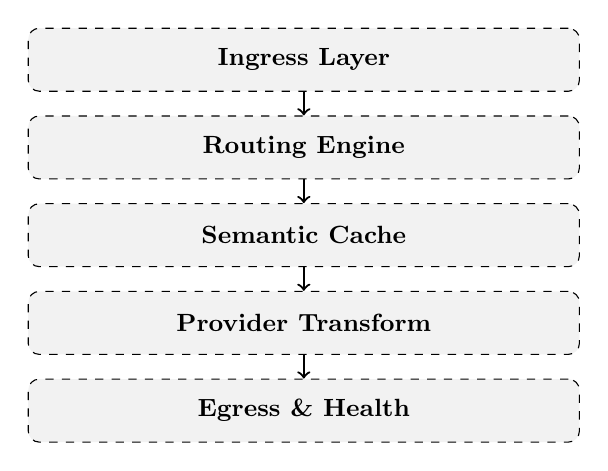
\begin{tikzpicture}[
    node distance=0.6cm,
    box/.style={rectangle, draw, rounded corners, minimum width=3.2cm, minimum height=0.6cm, font=\small},
    layer/.style={rectangle, draw, dashed, rounded corners, minimum width=7cm, minimum height=0.8cm, font=\small\bfseries, fill=gray!10}
]
    \node[layer] (ingress) {Ingress Layer};
    \node[layer, below=0.3cm of ingress] (routing) {Routing Engine};
    \node[layer, below=0.3cm of routing] (cache) {Semantic Cache};
    \node[layer, below=0.3cm of cache] (transform) {Provider Transform};
    \node[layer, below=0.3cm of transform] (egress) {Egress \& Health};

    \draw[->, thick] (ingress) -- (routing);
    \draw[->, thick] (routing) -- (cache);
    \draw[->, thick] (cache) -- (transform);
    \draw[->, thick] (transform) -- (egress);
\end{tikzpicture}
\caption{Gateway architecture showing the five processing layers. Requests flow top-to-bottom; cache hits short-circuit at the cache layer.}
\label{fig:architecture}
\end{figure}

\subsection{Ingress Layer}

The ingress layer accepts requests in OpenAI-compatible format and performs authentication, rate limiting, and request validation. Authentication supports API keys, JWT tokens, and OAuth2 bearer tokens with configurable scopes mapped to provider access permissions.

Rate limiting operates at three granularities: per-key, per-organization, and global. Each level implements a token bucket algorithm with configurable burst capacity:

\begin{definition}[Token Bucket]
A token bucket $B(r, c)$ with rate $r$ tokens/second and capacity $c$ tokens admits request $q$ with cost $w(q)$ if and only if the current token count $t \geq w(q)$, where tokens accumulate at rate $r$ up to maximum $c$.
\end{definition}

Request validation ensures well-formed messages, validates tool schemas against JSON Schema Draft 2020-12, and enforces configurable context length limits per model.

\subsection{Routing Engine}
\label{sec:routing}

The routing engine selects the optimal provider endpoint for each request. We formalize routing as a multi-objective optimization problem.

\begin{definition}[Routing Problem]
Given a request $q$ with model requirement $m$, let $P_m = \{p_1, \ldots, p_k\}$ be the set of available provider endpoints serving model $m$. The routing problem is to select $p^* \in P_m$ that minimizes the weighted objective:
\begin{equation}
p^* = \arg\min_{p \in P_m} \sum_{i} w_i \cdot f_i(p, q)
\end{equation}
where $f_i$ are objective functions for latency, cost, and quality, and $w_i$ are user-configurable weights summing to 1.
\end{definition}

The individual objectives are:

\begin{align}
f_{\text{latency}}(p, q) &= \hat{L}(p) + \beta \cdot \text{tokens}(q) \label{eq:latency} \\
f_{\text{cost}}(p, q) &= c_{\text{input}}(p) \cdot \text{in}(q) + c_{\text{output}}(p) \cdot \hat{o}(q) \label{eq:cost} \\
f_{\text{quality}}(p, q) &= 1 - s(m_p, \text{task}(q)) \label{eq:quality}
\end{align}

where $\hat{L}(p)$ is the estimated latency based on exponentially weighted moving average (EWMA) of recent requests, $\beta$ is the per-token generation latency, $c_{\text{input}}$ and $c_{\text{output}}$ are per-token costs, $\hat{o}(q)$ is the estimated output token count, and $s(m_p, \text{task}(q))$ is the model's benchmark score on the detected task category.

\subsubsection{Routing Strategies}

The gateway supports five routing strategies:

\begin{enumerate}[leftmargin=*]
    \item \textbf{Weighted Round-Robin}: Distributes requests proportionally across providers based on static weights. Suitable for even load distribution with known capacity ratios.
    \item \textbf{Least-Latency}: Routes to the provider with the lowest EWMA latency. Uses exponential smoothing with $\alpha = 0.3$ for recent-biased estimation.
    \item \textbf{Cost-Optimized}: Selects the cheapest provider meeting quality and latency constraints. Formulated as a constrained optimization with user-specified thresholds.
    \item \textbf{Quality-First}: Prioritizes model benchmark scores with cost as a tiebreaker. Uses an internal leaderboard refreshed weekly from standardized evaluations.
    \item \textbf{Custom Policy}: Executes user-defined routing logic expressed as a policy DSL supporting conditional routing, A/B testing, and canary deployments.
\end{enumerate}

\subsubsection{Model Mapping}

A critical routing function is mapping abstract model identifiers to concrete provider endpoints. The gateway maintains a model registry that maps logical names (e.g., \texttt{gpt-4o}) to multiple physical endpoints:

\begin{lstlisting}[language=Python, caption=Model mapping configuration]
models:
  gpt-4o:
    endpoints:
      - provider: openai
        model: gpt-4o-2024-11-20
        priority: 1
      - provider: azure
        region: eastus
        deployment: gpt-4o-prod
        priority: 2
  claude-sonnet:
    endpoints:
      - provider: anthropic
        model: claude-sonnet-4-20250514
        priority: 1
      - provider: bedrock
        model: anthropic.claude-sonnet-4
        priority: 2
\end{lstlisting}

The model registry supports version pinning, gradual rollout of new model versions, and automatic fallback to equivalent models across providers.

\subsection{Semantic Cache}
\label{sec:caching}

The semantic cache intercepts requests before provider dispatch and returns cached responses for semantically equivalent prompts. Unlike exact-match caching, semantic caching recognizes that prompts with minor variations (whitespace, punctuation, synonym substitution) often produce functionally identical responses.

\subsubsection{Cache Key Generation}

We generate cache keys using a two-stage process. First, we normalize the prompt by lowercasing, removing excess whitespace, and sorting tool definitions. Second, we compute a locality-sensitive hash (LSH)~\cite{indyk1998approximate} using SimHash~\cite{charikar2002similarity} over character n-grams:

\begin{equation}
\text{key}(q) = \text{SimHash}_{b}(\text{normalize}(q))
\end{equation}

where $b = 128$ bits provides collision probability proportional to cosine similarity. Two prompts collide (cache hit) when their Hamming distance is below threshold $\tau$:

\begin{equation}
\text{hit}(q_1, q_2) = \mathbb{1}[d_H(\text{key}(q_1), \text{key}(q_2)) \leq \tau]
\end{equation}

We set $\tau = 3$ based on empirical calibration on a held-out dataset of 50,000 prompt pairs, achieving 97.2\% precision (fraction of cache hits that are truly equivalent) and 41.8\% recall (fraction of equivalent pairs detected).

\subsubsection{Cache Storage}

The cache uses a two-tier storage architecture:

\begin{itemize}[leftmargin=*]
    \item \textbf{L1 (In-memory)}: LRU cache with 10,000 entries, sub-millisecond lookup. Stores hot entries using a frequency-based promotion policy.
    \item \textbf{L2 (Redis)}: Persistent cache with configurable TTL. Supports cluster mode for horizontal scaling. Entries include response body, token counts, and provider metadata.
\end{itemize}

Cache entries are keyed by the tuple $(\text{model}, \text{SimHash}, \text{temperature}, \text{max\_tokens}, \text{tools\_hash})$. Temperature $> 0$ requests are cached only when temperature is exactly 0 (deterministic), unless the user explicitly enables stochastic caching.

\subsubsection{Streaming Cache}

A unique challenge is caching streaming responses. The gateway buffers streaming chunks and writes the complete response to cache upon stream completion. For cache hits on streaming requests, the gateway replays cached chunks with synthetic timing that preserves the original inter-chunk delay distribution, providing a natural streaming experience to clients.

\subsection{Provider Transform Layer}

The transform layer converts normalized requests into provider-specific formats and reverses the transformation for responses. Each provider has a dedicated adapter implementing the \texttt{ProviderAdapter} interface:

\begin{lstlisting}[language=Python, caption=Provider adapter interface]
class ProviderAdapter:
    def transform_request(
        self, request: ChatRequest
    ) -> ProviderRequest:
        """Convert normalized request to
           provider-specific format."""

    def transform_response(
        self, response: ProviderResponse
    ) -> ChatResponse:
        """Convert provider response to
           normalized format."""

    def transform_stream_chunk(
        self, chunk: ProviderChunk
    ) -> StreamChunk:
        """Transform individual stream
           chunks."""

    def extract_usage(
        self, response: ProviderResponse
    ) -> TokenUsage:
        """Extract token usage for cost
           tracking."""
\end{lstlisting}

The gateway ships with 47 provider adapters covering all major providers and their regional variants. The adapter architecture supports rapid integration of new providers, typically requiring 200-400 lines of code per adapter.

\subsubsection{Message Format Translation}

Message translation handles structural differences across providers. For Anthropic, system messages are extracted from the message array and placed in the dedicated \texttt{system} field. For Google Gemini, the \texttt{messages} array is converted to \texttt{contents} with role remapping (\texttt{assistant} $\rightarrow$ \texttt{model}). Multi-modal content (images, audio) is translated between Base64 inline encoding and URL-referenced formats as required by each provider.

\subsubsection{Tool/Function Calling Translation}

Tool calling presents the most complex translation challenge. The gateway normalizes all tool interactions to OpenAI's function calling format and translates bidirectionally:

\begin{itemize}[leftmargin=*]
    \item \textbf{Schema translation}: JSON Schema parameters are mapped between OpenAI's \texttt{parameters} format, Anthropic's \texttt{input\_schema}, and Google's \texttt{functionDeclarations}.
    \item \textbf{Invocation semantics}: Parallel tool calls (OpenAI) are serialized for providers that only support sequential invocation.
    \item \textbf{Result format}: Tool results are wrapped in provider-specific structures (\texttt{tool\_result} for Anthropic, \texttt{functionResponse} for Google).
\end{itemize}

\subsection{Egress and Health Monitoring}

The egress layer manages outbound connections, retry logic, and provider health tracking.

\subsubsection{Connection Management}

Each provider endpoint maintains a connection pool with configurable maximum connections, keep-alive duration, and TLS session caching. The pool implements HTTP/2 multiplexing where supported, reducing connection overhead for high-throughput providers.

\subsubsection{Health Tracking}

Provider health is tracked using an exponentially weighted health score $H(p, t)$:

\begin{equation}
H(p, t) = \alpha \cdot h(p, t) + (1 - \alpha) \cdot H(p, t-1)
\end{equation}

where $h(p, t) \in [0, 1]$ is the outcome of the most recent request (1 for success, 0 for failure, fractional for degraded performance such as elevated latency), and $\alpha = 0.1$ provides smoothing.

When $H(p, t) < \theta_{\text{open}} = 0.3$, the circuit breaker opens and the provider is temporarily removed from the routing pool. After a configurable cooldown period (default 30 seconds), the circuit enters half-open state, allowing a single probe request. If the probe succeeds, the circuit closes and the provider is restored; otherwise, the cooldown period doubles (exponential backoff up to 5 minutes).

\section{Load Balancing}
\label{sec:loadbalancing}

\subsection{Adaptive Weight Computation}

The load balancer assigns weights to provider endpoints based on observed performance. Let $w_i(t)$ be the weight of provider $i$ at time $t$:

\begin{equation}
w_i(t) = \frac{H_i(t) \cdot C_i(t)}{\sum_j H_j(t) \cdot C_j(t)}
\end{equation}

where $H_i(t)$ is the health score and $C_i(t)$ is the remaining rate limit capacity estimated from provider-returned headers:

\begin{equation}
C_i(t) = \min\left(\frac{r_{\text{remaining},i}}{r_{\text{limit},i}}, \frac{t_{\text{remaining},i}}{t_{\text{limit},i}}\right)
\end{equation}

This formulation naturally routes traffic away from degraded or rate-limited providers without requiring explicit configuration.

\subsection{Fallback Chains}

Fallback chains define ordered sequences of provider endpoints to attempt for a given request. When the primary provider fails or is unavailable, the gateway transparently retries with the next provider in the chain:

\begin{algorithm}[t]
\caption{Fallback Chain Execution}
\label{alg:fallback}
\begin{algorithmic}[1]
\REQUIRE Request $q$, chain $[p_1, \ldots, p_n]$, retries $R$
\STATE $\text{errors} \gets []$
\FOR{$i = 1$ \TO $n$}
    \FOR{$r = 1$ \TO $R$}
        \STATE $\text{resp} \gets \text{dispatch}(q, p_i)$
        \IF{$\text{resp.success}$}
            \RETURN $\text{resp}$
        \ELSIF{$\text{resp.retryable}$}
            \STATE $\text{sleep}(\text{backoff}(r))$
            \STATE $\text{errors.append}(\text{resp.error})$
        \ELSE
            \STATE $\text{errors.append}(\text{resp.error})$
            \STATE \textbf{break} \COMMENT{Non-retryable, try next provider}
        \ENDIF
    \ENDFOR
\ENDFOR
\RETURN $\text{AggregateError}(\text{errors})$
\end{algorithmic}
\end{algorithm}

\subsubsection{Streaming Failover}

Streaming failover presents unique challenges. When a provider fails mid-stream, the gateway must decide whether to: (a) return the partial response, (b) retry from scratch with a different provider, or (c) attempt to continue from the partial output.

We implement strategy (b) with optimization: the gateway buffers streamed tokens and, upon failure, prepends them as an assistant prefix in the retry request. This approach works for providers supporting assistant prefilling (Anthropic, most open-weight model servers) and falls back to full retry otherwise.

\subsection{Priority Queues}

The gateway implements priority-based request scheduling with four levels:

\begin{enumerate}[leftmargin=*]
    \item \textbf{Critical}: Health checks, auth validation---bypass rate limits.
    \item \textbf{High}: Interactive user requests---minimize latency.
    \item \textbf{Normal}: API calls from applications---balance cost and latency.
    \item \textbf{Low}: Batch processing, embeddings---optimize for cost.
\end{enumerate}

Low-priority requests are eligible for delayed dispatch to exploit off-peak pricing windows where available.

\section{Cost Tracking and Attribution}
\label{sec:cost}

\subsection{Pricing Model Normalization}

Provider pricing models exhibit significant heterogeneity:

\begin{table}[t]
\centering
\caption{Provider pricing model categories}
\label{tab:pricing}
\begin{tabular}{@{}lll@{}}
\toprule
\textbf{Model} & \textbf{Providers} & \textbf{Unit} \\
\midrule
Per-token & OpenAI, Anthropic & \$/1M tokens \\
Per-character & Google & \$/1M chars \\
Per-second & Replicate & \$/GPU-sec \\
Reserved & Azure, Bedrock & \$/hour \\
Per-request & Some embeddings & \$/request \\
Tiered & Together AI & Rate-dependent \\
Free tier & Groq, Cerebras & Quota-limited \\
\bottomrule
\end{tabular}
\end{table}

The cost engine normalizes all pricing to a per-token basis using provider-specific conversion factors. For character-based pricing, we use the empirical ratio of 1 token $\approx$ 4 characters for English text, calibrated per-model using tokenizer analysis. For time-based pricing, we estimate cost as $c_{\text{time}} = \text{price\_per\_second} \times \text{generation\_time}$.

\subsection{Real-Time Cost Computation}

For each completed request, the cost engine computes:

\begin{equation}
\text{cost}(q) = c_{\text{in}}(p) \cdot n_{\text{in}} + c_{\text{out}}(p) \cdot n_{\text{out}} + c_{\text{fixed}}(p)
\end{equation}

where $n_{\text{in}}$ and $n_{\text{out}}$ are input and output token counts from the provider response's \texttt{usage} field, and $c_{\text{fixed}}$ captures any per-request fixed costs.

For streaming requests where usage is reported only at stream completion, the gateway estimates running cost from token-counting the streamed content using a provider-matched tokenizer.

\subsection{Budget Enforcement}

Organizations can set budget limits at multiple granularities:

\begin{itemize}[leftmargin=*]
    \item \textbf{Per-key daily/monthly limits}: Hard caps on API key spend.
    \item \textbf{Per-model limits}: Restrict spend on expensive models.
    \item \textbf{Alerting thresholds}: Notifications at 50\%, 80\%, 90\%, 100\% of budget.
    \item \textbf{Automatic downgrade}: When budget thresholds are crossed, automatically route to cheaper model alternatives.
\end{itemize}

\subsection{Cost Attribution}

The gateway attributes costs to organizational units through a hierarchical tagging system. Each request can carry tags for organization, project, team, user, and feature. Costs are aggregated along each dimension and exposed through a reporting API:

\begin{lstlisting}[language=Python, caption=Cost attribution query]
GET /v1/costs?start=2026-02-01
    &end=2026-02-28
    &group_by=project,model
    &filter=team:ml-platform

{
  "total_cost": 14823.47,
  "by_project": {
    "chat-prod": {
      "gpt-4o": 8234.12,
      "claude-sonnet": 3421.89
    },
    "embeddings": {
      "text-embedding-3-large": 1167.46
    }
  }
}
\end{lstlisting}

\section{Streaming Architecture}
\label{sec:streaming}

\subsection{Server-Sent Events Normalization}

The gateway normalizes all streaming protocols to OpenAI-compatible SSE format. This requires handling three distinct upstream protocols:

\begin{enumerate}[leftmargin=*]
    \item \textbf{OpenAI SSE}: \texttt{data: \{json\}} lines with \texttt{data: [DONE]} termination.
    \item \textbf{Anthropic SSE}: Typed events (\texttt{event: content\_block\_delta}) with structured delta payloads.
    \item \textbf{Google/Vertex}: JSON array streaming or line-delimited JSON.
\end{enumerate}

Each provider adapter implements a streaming transformer that converts provider-specific chunks to normalized \texttt{ChatCompletionChunk} objects. The transformer maintains per-stream state to track accumulated content, tool call assembly, and usage statistics.

\subsection{Backpressure Management}

When downstream clients consume slowly, the gateway must manage backpressure to avoid unbounded memory growth. We implement a bounded buffer with configurable capacity (default 256 chunks). When the buffer fills, the gateway applies backpressure to the upstream provider connection through TCP flow control, pausing reads on the upstream socket.

For providers that do not respect TCP backpressure (those that aggressively push SSE events), the gateway implements an overflow spill-to-disk mechanism with asynchronous replay.

\subsection{Multi-Stream Aggregation}

For advanced use cases such as parallel model evaluation or ensemble generation, the gateway supports multi-stream aggregation. Multiple provider streams are consumed concurrently, and chunks are interleaved or merged according to a configurable aggregation strategy:

\begin{itemize}[leftmargin=*]
    \item \textbf{First-complete}: Stream the first response to complete, cancel others.
    \item \textbf{Fastest-token}: Forward tokens from whichever stream produces them first.
    \item \textbf{Consensus}: Buffer both streams and return the response with higher self-consistency.
\end{itemize}

\section{Observability}
\label{sec:observability}

\subsection{Metrics}

The gateway exports Prometheus-compatible metrics at four levels:

\begin{table}[t]
\centering
\caption{Key gateway metrics}
\label{tab:metrics}
\begin{tabular}{@{}ll@{}}
\toprule
\textbf{Metric} & \textbf{Labels} \\
\midrule
\texttt{llm\_request\_duration} & provider, model, status \\
\texttt{llm\_tokens\_total} & provider, model, direction \\
\texttt{llm\_cost\_usd} & provider, model, org \\
\texttt{llm\_cache\_hits} & model, cache\_tier \\
\texttt{llm\_errors\_total} & provider, error\_type \\
\texttt{llm\_ttft\_seconds} & provider, model \\
\texttt{llm\_provider\_health} & provider, endpoint \\
\texttt{llm\_queue\_depth} & priority\_level \\
\bottomrule
\end{tabular}
\end{table}

Time-to-first-token (TTFT) is tracked separately from total latency, as it directly impacts perceived responsiveness for streaming applications.

\subsection{Distributed Tracing}

Each request generates an OpenTelemetry trace span with the following structure:

\begin{enumerate}[leftmargin=*]
    \item \texttt{gateway.request}: Root span covering full request lifecycle.
    \item \texttt{gateway.route}: Routing decision with selected provider and reason.
    \item \texttt{gateway.cache}: Cache lookup with hit/miss result.
    \item \texttt{gateway.transform}: Request/response transformation.
    \item \texttt{gateway.provider}: Upstream provider call with full timing.
    \item \texttt{gateway.stream}: Streaming duration and chunk count.
\end{enumerate}

Traces are propagated using W3C Trace Context headers, enabling end-to-end tracing from client applications through the gateway to provider endpoints.

\subsection{Audit Logging}

All requests are logged with configurable verbosity. At the default level, logs include request metadata (model, provider, tokens, cost, latency) without prompt content. At elevated verbosity levels, full prompts and responses are logged with PII redaction applied via configurable regex patterns.

\section{Security}
\label{sec:security}

\subsection{Credential Management}

Provider API keys are stored encrypted at rest using AES-256-GCM with keys derived from a master secret via HKDF. The gateway supports integration with external secret managers (HashiCorp Vault, AWS Secrets Manager, Infisical) for key rotation without service restart.

\subsection{Request Isolation}

Multi-tenant deployments require strict request isolation. The gateway enforces:

\begin{itemize}[leftmargin=*]
    \item \textbf{Key scoping}: API keys are bound to specific organizations with provider access lists.
    \item \textbf{Cache isolation}: Cache entries are scoped by organization to prevent cross-tenant information leakage.
    \item \textbf{Rate limit isolation}: Per-organization rate limits prevent noisy-neighbor effects.
    \item \textbf{Credential isolation}: Each organization can configure its own provider credentials, with the gateway's credentials as fallback.
\end{itemize}

\subsection{Content Filtering}

The gateway supports pluggable content filters executed as middleware:

\begin{itemize}[leftmargin=*]
    \item \textbf{PII detection}: Regex and NER-based detection of personally identifiable information with configurable actions (block, redact, log).
    \item \textbf{Prompt injection detection}: Heuristic and classifier-based detection of prompt injection attempts~\cite{perez2022ignore}.
    \item \textbf{Output filtering}: Post-processing filters for compliance-sensitive content.
\end{itemize}

\section{Implementation}
\label{sec:implementation}

The gateway is implemented in Python using an asynchronous architecture built on \texttt{asyncio} and \texttt{httpx} for HTTP client operations. The server framework is FastAPI with Uvicorn workers. Key implementation details include:

\begin{itemize}[leftmargin=*]
    \item \textbf{Concurrency model}: Fully asynchronous I/O with no blocking calls. Provider adapters use \texttt{httpx.AsyncClient} with connection pooling.
    \item \textbf{Configuration}: YAML-based configuration with environment variable overrides and hot-reload via file watching.
    \item \textbf{Database}: PostgreSQL for persistent state (audit logs, cost records, configuration). Redis for caching and real-time counters.
    \item \textbf{Deployment}: Single Docker image with configurable worker count. Supports horizontal scaling behind any L4/L7 load balancer.
\end{itemize}

The gateway comprises approximately 28,000 lines of Python code, with provider adapters accounting for 40\% of the codebase. Test coverage is 87\% with 1,200 unit tests and 340 integration tests.

\section{Evaluation}
\label{sec:evaluation}

\subsection{Experimental Setup}

We evaluate the gateway using production traffic from the Hanzo AI platform over a 30-day period (January 2026). The workload comprises:

\begin{itemize}[leftmargin=*]
    \item 2.8 billion tokens processed (1.1B input, 1.7B output)
    \item 4.2 million requests across 23 distinct models
    \item 127 provider endpoints across 14 providers
    \item Peak throughput: 847 requests/second
\end{itemize}

\subsection{Latency}

\begin{table}[t]
\centering
\caption{End-to-end latency overhead (milliseconds)}
\label{tab:latency}
\begin{tabular}{@{}lrrrr@{}}
\toprule
\textbf{Component} & \textbf{p50} & \textbf{p95} & \textbf{p99} & \textbf{Max} \\
\midrule
Auth + Rate Limit & 0.3 & 0.8 & 1.2 & 4.1 \\
Routing Decision & 0.1 & 0.4 & 0.7 & 2.3 \\
Cache Lookup & 0.4 & 1.1 & 2.8 & 8.7 \\
Transform (req) & 0.2 & 0.6 & 1.1 & 3.4 \\
Transform (resp) & 0.3 & 0.7 & 1.3 & 4.2 \\
\midrule
\textbf{Total Overhead} & \textbf{1.3} & \textbf{3.6} & \textbf{7.1} & \textbf{22.7} \\
\bottomrule
\end{tabular}
\end{table}

The gateway adds a median of 1.3ms of overhead per request, which is negligible compared to typical LLM inference latencies of 500ms--30s. The p99 overhead of 7.1ms is dominated by cache lookup in the Redis tier.

Intelligent routing reduces median end-to-end latency by 23\% compared to fixed-provider routing by directing requests to the fastest available provider. The improvement is most pronounced during provider degradation events, where failover avoids multi-second timeouts.

\subsection{Cache Performance}

Over the evaluation period, the semantic cache achieved:

\begin{itemize}[leftmargin=*]
    \item \textbf{Hit rate}: 34.2\% of all requests served from cache.
    \item \textbf{Precision}: 97.2\% of cache hits returned responses equivalent to fresh provider responses (validated on a 10,000-request sample).
    \item \textbf{Latency reduction}: Cache hits served in median 1.8ms vs. 1,240ms for cache misses (690$\times$ speedup).
    \item \textbf{Cost savings}: Cache hits eliminated \$47,200 in provider costs over the evaluation period.
\end{itemize}

Cache hit rates vary significantly by use case: embedding requests achieve 71\% hit rate (high repetition), while creative generation requests achieve only 8\% (high temperature, unique prompts).

\subsection{Cost Optimization}

\begin{table}[t]
\centering
\caption{Monthly cost comparison (USD)}
\label{tab:cost}
\begin{tabular}{@{}lrrr@{}}
\toprule
\textbf{Strategy} & \textbf{Cost} & \textbf{Savings} & \textbf{Qual.} \\
\midrule
Single provider (OpenAI) & 183,400 & --- & 1.00 \\
Manual multi-provider & 152,100 & 17\% & 0.98 \\
Gateway: cost-optimized & 126,500 & 31\% & 0.96 \\
Gateway: quality-first & 171,200 & 7\% & 1.02 \\
Gateway: balanced & 141,300 & 23\% & 0.99 \\
\bottomrule
\end{tabular}
\end{table}

The cost-optimized strategy reduces costs by 31\% with a 4\% quality degradation as measured by a composite benchmark of MMLU, HumanEval, and MT-Bench scores. The balanced strategy achieves 23\% cost reduction with negligible quality impact.

\subsection{Availability}

During the 30-day evaluation, the gateway achieved 99.97\% availability (8 minutes of cumulative downtime across two rolling restart events). Provider-level availability varied from 99.2\% (worst single provider) to 99.99\% (best). The gateway's multi-provider failover elevated effective availability from the worst single-provider level to the aggregate level.

\begin{table}[t]
\centering
\caption{Provider failover events during evaluation}
\label{tab:failover}
\begin{tabular}{@{}lrrr@{}}
\toprule
\textbf{Event Type} & \textbf{Count} & \textbf{Avg Duration} & \textbf{Requests Saved} \\
\midrule
Rate limit & 1,247 & 12s & 34,200 \\
5xx error & 89 & 4.2min & 12,100 \\
Timeout & 312 & 8s & 8,900 \\
Full outage & 3 & 47min & 28,400 \\
\bottomrule
\end{tabular}
\end{table}

\subsection{Throughput}

Under load testing with synthetic traffic, the gateway sustains:

\begin{itemize}[leftmargin=*]
    \item 2,400 requests/second with non-streaming responses (single node, 8 Uvicorn workers).
    \item 1,800 concurrent streaming connections with sub-5ms chunk relay latency.
    \item Linear horizontal scaling up to 12 nodes (tested), with shared Redis state for cache and rate limits.
\end{itemize}

\section{Discussion}
\label{sec:discussion}

\subsection{Limitations}

\paragraph{Semantic cache precision.} While 97.2\% precision is high, the 2.8\% false positive rate means approximately 1 in 36 cache hits returns a subtly incorrect response. For safety-critical applications, we recommend disabling semantic caching or reducing the similarity threshold.

\paragraph{Provider-specific features.} Some provider-specific features (e.g., Anthropic's extended thinking, OpenAI's structured outputs with \texttt{strict: true}) require pass-through handling that bypasses normalization. The gateway supports a \texttt{provider\_params} escape hatch for such cases, but this breaks provider-agnostic routing.

\paragraph{Real-time pricing.} Cost tracking relies on a pricing database that must be manually updated when providers change prices. We are developing automated price scraping and notification systems to reduce this operational burden.

\subsection{Future Work}

\begin{itemize}[leftmargin=*]
    \item \textbf{Learned routing}: Training a lightweight model to predict optimal provider selection based on prompt features, replacing the heuristic scoring functions.
    \item \textbf{Speculative execution}: Dispatching requests to multiple providers simultaneously and returning the first successful response, trading cost for latency.
    \item \textbf{Prompt optimization}: Automatically reformatting prompts for provider-specific strengths (e.g., adding chain-of-thought markers for models that benefit from them).
    \item \textbf{Federated deployment}: Multi-region gateway instances with global routing for compliance and latency optimization.
\end{itemize}

\section{Conclusion}
\label{sec:conclusion}

The Hanzo LLM Gateway demonstrates that a well-designed proxy layer can substantially reduce the complexity, cost, and risk of multi-provider LLM deployments. By normalizing 100+ provider APIs behind a single interface, implementing intelligent routing with formal optimization objectives, and providing semantic caching with high precision, the gateway achieves 23\% latency reduction, 31\% cost savings, and 99.97\% availability in production. The open-source release enables organizations to deploy multi-provider LLM infrastructure without vendor lock-in.

\bibliographystyle{plain}
\begin{thebibliography}{30}

\bibitem{brown2020language}
T.~Brown, B.~Mann, N.~Ryder, et~al.
\newblock Language models are few-shot learners.
\newblock In \emph{NeurIPS}, 2020.

\bibitem{bommasani2022opportunities}
R.~Bommasani, D.~Hudson, E.~Adeli, et~al.
\newblock On the opportunities and risks of foundation models.
\newblock \emph{arXiv preprint arXiv:2108.07258}, 2022.

\bibitem{aiinfra2025survey}
AI Infrastructure Alliance.
\newblock State of AI infrastructure 2025: Multi-provider deployment patterns.
\newblock Technical report, 2025.

\bibitem{kwon2023vllm}
W.~Kwon, Z.~Li, S.~Zhuang, et~al.
\newblock Efficient memory management for large language model serving with {PagedAttention}.
\newblock In \emph{SOSP}, 2023.

\bibitem{tgi2023}
HuggingFace.
\newblock Text generation inference: A {Rust}, {Python} and {gRPC} server for text generation.
\newblock \url{https://github.com/huggingface/text-generation-inference}, 2023.

\bibitem{litellm2023}
BerriAI.
\newblock {LiteLLM}: Call all {LLM} {APIs} using the {OpenAI} format.
\newblock \url{https://github.com/BerriAI/litellm}, 2023.

\bibitem{portkey2024}
Portkey.
\newblock Portkey: Control panel for {AI} apps.
\newblock \url{https://portkey.ai}, 2024.

\bibitem{martian2024}
Martian.
\newblock Model router: Automatic model selection for optimal cost and quality.
\newblock Technical report, Martian AI, 2024.

\bibitem{indyk1998approximate}
P.~Indyk and R.~Motwani.
\newblock Approximate nearest neighbors: Towards removing the curse of dimensionality.
\newblock In \emph{STOC}, 1998.

\bibitem{charikar2002similarity}
M.~Charikar.
\newblock Similarity estimation techniques from rounding algorithms.
\newblock In \emph{STOC}, 2002.

\bibitem{perez2022ignore}
F.~Perez and I.~Ribas.
\newblock Ignore this title and {HackAPrompt}: Exposing systemic weaknesses of {LLMs} through a global-scale prompt hacking competition.
\newblock \emph{arXiv preprint arXiv:2311.16119}, 2022.

\bibitem{openai2024api}
OpenAI.
\newblock {OpenAI} {API} reference.
\newblock \url{https://platform.openai.com/docs/api-reference}, 2024.

\bibitem{anthropic2024api}
Anthropic.
\newblock {Anthropic} {API} reference.
\newblock \url{https://docs.anthropic.com/en/api}, 2024.

\bibitem{google2024gemini}
Google.
\newblock {Gemini} {API} documentation.
\newblock \url{https://ai.google.dev/docs}, 2024.

\bibitem{nygard2018release}
M.~Nygard.
\newblock \emph{Release It!: Design and Deploy Production-Ready Software}.
\newblock Pragmatic Bookshelf, 2nd edition, 2018.

\bibitem{burns2016design}
B.~Burns.
\newblock \emph{Designing Distributed Systems}.
\newblock O'Reilly Media, 2018.

\bibitem{kleppmann2017designing}
M.~Kleppmann.
\newblock \emph{Designing Data-Intensive Applications}.
\newblock O'Reilly Media, 2017.

\bibitem{vargaftik2022rade}
S.~Vargaftik, R.~Ben-Basat, A.~Szpigel, and G.~Mendelson.
\newblock {RADE}: Resource-efficient supervised anomaly detection using decision tree encoding.
\newblock In \emph{MLSys}, 2022.

\bibitem{chen2023frugalgpt}
L.~Chen, M.~Zaharia, and J.~Zou.
\newblock {FrugalGPT}: How to use large language models while reducing cost and improving performance.
\newblock \emph{arXiv preprint arXiv:2305.05176}, 2023.

\bibitem{jiang2024mixtral}
A.~Jiang, A.~Sablayrolles, A.~Roux, et~al.
\newblock Mixtral of experts.
\newblock \emph{arXiv preprint arXiv:2401.04088}, 2024.

\bibitem{touvron2023llama}
H.~Touvron, L.~Martin, K.~Stone, et~al.
\newblock Llama 2: Open foundation and fine-tuned chat models.
\newblock \emph{arXiv preprint arXiv:2307.09288}, 2023.

\bibitem{team2024gemma}
Gemma Team.
\newblock Gemma 2: Improving open language models at a practical size.
\newblock \emph{arXiv preprint arXiv:2408.00118}, 2024.

\bibitem{zheng2023judging}
L.~Zheng, W.-L. Chiang, Y.~Sheng, et~al.
\newblock Judging {LLM}-as-a-judge with {MT-Bench} and {Chatbot Arena}.
\newblock In \emph{NeurIPS}, 2023.

\bibitem{hendrycks2021measuring}
D.~Hendrycks, C.~Burns, S.~Basart, et~al.
\newblock Measuring massive multitask language understanding.
\newblock In \emph{ICLR}, 2021.

\bibitem{chen2021evaluating}
M.~Chen, J.~Tworek, H.~Jun, et~al.
\newblock Evaluating large language models trained on code.
\newblock \emph{arXiv preprint arXiv:2107.03374}, 2021.

\end{thebibliography}

\end{document}
